\documentclass[epsfig,10pt,fullpage]{article} \addtolength{\textwidth}{1.5in}
\addtolength{\oddsidemargin}{-0.75in}
\addtolength{\topmargin}{-0.75in}
\addtolength{\textheight}{1.5in}
\addtolength{\evensidemargin}{0.75in}
\raggedbottom
\usepackage{ae,aecompl}
\usepackage{epsfig,float,times}
\usepackage{graphicx}
\usepackage{hyperref}
\usepackage[usenames]{xcolor}

\hypersetup{
    colorlinks=true,
    linkcolor=blue,
    filecolor=magenta,      
    urlcolor=blue,
    pdftitle={Sharelatex Example},
    bookmarks=true,
    pdfpagemode=FullScreen,
}
\newcommand{\red}[1]{{\color{red}\sf{#1}}}
\newcommand{\blue}[1]{{\color{blue}\sf{#1}}}

\usepackage{placeins}
\usepackage{listings}
\definecolor{PineGreen}{rgb}{0.0, 0.47, 0.44}
\definecolor{ForestGreen}{rgb}{0.13, 0.55, 0.13}
\definecolor{Brown}{rgb}{0.59, 0.29, 0.0}

\lstdefinelanguage{ASM}{
  morekeywords =
  [1]{mv,mvt,add,sub,st,ld,and,b,bne,beq,bcc,bcs,bpl,bmi,bl,push,pop,cmp,lsl,lsr,asr,ror},
  morekeywords = [2]{word, define},
  keywordstyle = [1]\color{ForestGreen},
  keywordstyle = [2]\color{blue},
  sensitive = true,
  morecomment = [l]{//},
}
\lstset{
%language = C,
%language = VHDL,
language = ASM,
basicstyle=\small\color{black}\ttfamily, commentstyle=\small\color{Brown}\itshape\ttfamily,
showstringspaces=false,
frame=none, %lines % boxed listings
breaklines=true,
breakatwhitespace=true,
tabsize=3
}
\setcounter{table}{4}
\setcounter{figure}{23}

\begin{document}
~\\
\centerline{\huge Laboratory Exercise 11}
~\\
\centerline{\large A More Enhanced Processor}
~\\
In Lab Exercise 10 you made enhancements to the processor from Lab 9, by including a
program counter, memory interface, and the \texttt{ld}, \texttt{st}, \texttt{and}, and
\texttt{b\{cond\}} instructions. This exercise involves
further extensions to the processor design. The numbering of 
figures and tables in this document are continued from those in Parts I to VII of Lab 
Exercises 9 and 10.

~\\
\noindent
For this exercise you will augment the processor architecture so that it supports
subroutines and stacks, and also provides shift and rotate operations. 
All of the processor registers will be the same as in Lab 10,
except that register $r5$ will be changed into an {\it up/down counter}, as illustrated 
in Figure~\ref{fig:figr6}. This figure shows only the processor 
registers $r4, \ldots, r7$ ({\it pc}) and their
connections to the {\it Buswires} multiplexer; refer to Lab~10 to see a more complete
schematic of the processor.

~\\
\noindent
In assembly-language code register $r5$ can be referred to as the {\it stack pointer} 
register, {\it sp}. It is used as an {\it address} for pushing and popping data on the stack. 
Since it is an up/down counter, the $sp$ can easily be
{\it decremented} before a register is {\it pushed} onto the stack, and {\it incremented} 
after a register has been {\it popped} off of the stack. The  processor's control unit 
decrements {\it sp} by using the {\it sp\_decr} signal shown in Figure~\ref{fig:figr6}, 
and increments this register by using the {\it sp\_incr} signal. These signals are just 
the {\it up}/{\it down} control inputs for the counter. Arbitrary data can also be 
loaded into register $r5$ ($sp$) in the same way as in Lab 10, by using the {\it r5}$_{in}$ signal.

~\\
\noindent
The processor will have eight new instructions, which are listed
in Table~\ref{tab:new_instr}. The \texttt{push rX} instruction is used to store the contents 
of a register, {\it rX}, onto the stack. This instruction first decrements the {\it sp} 
(register $r5$), and then stores {\it rX} into memory at the address in {\it sp}. The
\texttt{pop rX} instruction is used to load data into a register {\it rX} from memory at 
the address in {\it sp}.  After loading this data, {\it sp} is then incremented.     

~\\
\noindent
The branch instruction, \texttt{b\{cond\}}, was introduced in Lab~10. This exercise defines a new
type of branch instruction, \texttt{bl Label},  which is used for {\it subroutine linkage}.
This {\it branch with link} instruction first copies the address of the program counter 
(which will already have been incremented to point to the {\it next} instruction after 
the \texttt{bl}), into register $r6$. Then, the \texttt{bl} instruction sets the program 
counter to the address of the subroutine, \texttt{Label}. 
In assembly-language code register $r6$ can be referred to as the {\it link register}, {\it lr}. 
To effect a {\it return}, a subroutine can use the instruction \texttt{mv~~pc, lr}.

\begin{figure}[t]
\begin{center}
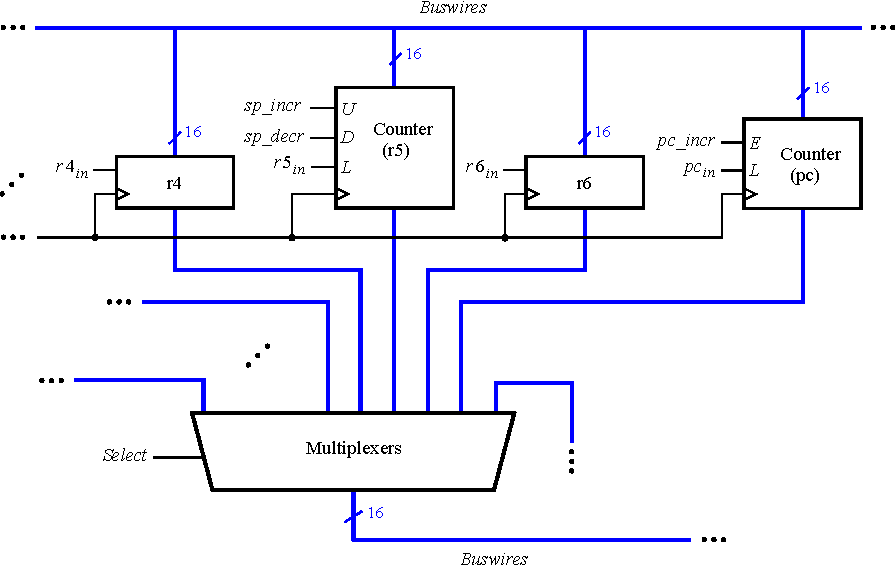
\includegraphics[scale = 0.8]{figures/r6.pdf}
\end{center}
\caption{The stack pointer register.}
\label{fig:figr6}
\end{figure}

\begin{table}[H]
\begin{center}
\begin{tabular}{l|l}
\rule[-0.075in]{0in}{0.25in}Operation & ~~Function performed \\ \hline 
\rule[-0.075in]{0in}{0.25in}{\it push}~~~{\it rX} & ~~{\it sp} $\leftarrow$ {\it sp} $-1$, [{\it sp}] $\leftarrow$ {\it rX}\\ 
\rule[-0.075in]{0in}{0.25in}{\it pop}~~~{\it rX} & ~~{\it rX} $\leftarrow$ [{\it sp}], {\it
sp} $\leftarrow$ {\it sp} $+1$  \\ 
\rule[-0.075in]{0in}{0.25in}{\it bl}~~~{\it Label} & ~~$r6$ $\leftarrow$ {\it pc}, {\it pc} $\leftarrow$ {\it Label} \\ 
\rule[-0.075in]{0in}{0.25in}{\it cmp}~~~{\it rX}, {\it Op2} & ~~performs {\it rX} $-$ {\it Op2}, sets flags \\ 
\rule[-0.075in]{0in}{0.25in}{\it lsl}~~~{\it rX}, {\it Op2} & ~~{\it rX} $\leftarrow$ {\it
rX} <\hspace{-.25mm}< {\it Op2}\\ 
\rule[-0.075in]{0in}{0.25in}{\it lsr}~~~{\it rX}, {\it Op2} & ~~{\it rX} $\leftarrow$ {\it
rX} >\hspace{-0.25mm}> {\it Op2}\\ 
\rule[-0.075in]{0in}{0.25in}{\it asr}~~~{\it rX}, {\it Op2} & ~~{\it rX} $\leftarrow$ {\it
rX} >\hspace{-0.25mm}>\hspace{-0.25mm}> {\it Op2}\\ 
\rule[-0.075in]{0in}{0.25in}{\it ror}~~~{\it rX}, {\it Op2} & ~~{\it rX} $\leftarrow$ {\it
rX} <\hspace{-0.25mm}<\hspace{-0.25mm}>\hspace{-0.25mm}> {\it Op2}\\ 
\end{tabular}
\caption{New instructions.}
\label{tab:new_instr}
\end{center}
\end{table}

\noindent
The \texttt{cmp} instruction is similar to the \texttt{sub} instruction that was introduced in 
Lab 9. This instruction performs the operation {\it rX} $-$ {\it Op2}, but only affects the
flags. The \texttt{cmp} instruction does not modify register {\it rX}. 

\noindent
Finally, the \texttt{lsl},
\texttt{lsr}, \texttt{asr}, and \texttt{ror} instructions extend the ALU in the processor to 
provide {\it shift} and {\it rotate} capability. The \texttt{lsl} instruction performs a
logical-shift-left operation (<\hspace{-.25mm}<). It shifts the
contents of register {\it rX} to the left by the amount specified in {\it Op2}. The effect
of this instruction is to perform {\it multiplication} by {\it powers of two}. The maximum 
possible shift amount is 15. It can be given in the form of immediate data, \#{\it D}, or in 
(the four least-significant bits of) another register, {\it rY}. The result produce by the
\texttt{lsl} instruction affects all of the processor's condition-code flags {\it z}, {\it n}, 
and {\it c}. The last bit shifted-left out of {\it rX} determines the value of the {\it c} flag. 

~\\
\noindent
The \texttt{lsr} instruction performs a logical-shift-right operation (>\hspace{-0.25mm}>).
This means that the
contents of register {\it rX} are shifted to the right by the amount specified in {\it Op2}, 
and each bit {\it shifted-in} has the value 0. The effect of this instruction is to
perform an {\it unsigned division} by powers of two. The shift amount is
specified in {\it Op2} in the same way as described previously for the \texttt{lsl} instruction. 
The \texttt{lsr} instruction affects all of the processor's condition-code flags 
{\it z}, {\it n}, and {\it c}, but the effect on the {\it c} flag is {\it undefined}.

~\\
\noindent
The \texttt{asr} instruction performs an arithmetic-shift-right operation 
(>\hspace{-0.25mm}>\hspace{-0.25mm}>). This means that the
contents of register {\it rX} are shifted to the right by the amount specified in {\it Op2}, 
and each bit {\it shifted-in} replicates the {\it sign-bit} of {\it rX}. The effect of 
this instruction is to perform a {\it signed division} by powers of two. The shift amount is
specified in {\it Op2} in the same way as described previously. The 
\texttt{asr} instruction affects all of the processor's condition-code flags {\it z}, {\it n}, 
and {\it c}, but the effect on the {\it c} flag is {\it undefined}.

~\\
\noindent
The \texttt{ror} instruction performs a rotate-right operation
(<\hspace{-0.25mm}<\hspace{-0.25mm}>\hspace{-0.25mm}>). It shifts the contents of
register {\it rX} to the right in a circular fashion, so that each bit shifted out of the
least-significant-bit of {\it rX} is shifted into the most-significant bit.  The shift amount is
specified in {\it Op2} in the same way as described previously. The 
\texttt{ror} instruction affects all of the processor's condition-code flags {\it z}, {\it n}, 
and {\it c}, but the effect on the {\it c} flag is {\it undefined}.

\subsection*{Instruction Encodings}
\noindent
Recall from Labs~9 and~10 that instructions are encoded using a 16-bit format. For instructions 
that have two operands, when {\it Op2} is a register the encoding is \texttt{III0XXX000000YYY}, 
and when {\it Op2} is an immediate \#{\it D} constant the format is \texttt{III1XXXDDDDDDDDD}. The
\texttt{ld} and \texttt{st} instructions are encoded as \texttt{1000XXX000000YYY} and
\texttt{1010XXX000000YYY}, respectively. You should encode the \texttt{pop} instruction 
similarly to \texttt{ld}, with the encoding \texttt{1001XXX000000101}. Also, encode 
\texttt{push} similarly to \texttt{st}, using the encoding \texttt{1011XXX000000101}.
Notice that for both \texttt{push} and \texttt{pop} the \texttt{YYY} field is hard-coded to 
correspond to the stack pointer register, $r5$. 

~\\
\noindent
Recall from Lab~10 that the \texttt{b\{cond\}} instruction uses the \texttt{XXX} field to
encode a {\it condition}, where \texttt{XXX} $= 000$ ({\it none}), 001 ({\it eq}), 010 
({\it ne}), and so on. Implement the \texttt{bl} instruction by using the previously-unassigned 
code \texttt{XXX}~$= 111$.   

~\\
\noindent
You should implement the \texttt{cmp} instruction similarly to the \texttt{add},
\texttt{sub}, and \texttt{and} instructions. Use the previously-unassigned code
\texttt{III = 111}; if {\it Op2} is a register, then \texttt{cmp} is encoded as
\texttt{1110XXX000000YYY}, and if {\it Op2} is \#{\it D}, then \texttt{cmp} is encoded 
as \texttt{1111XXXDDDDDDDDD}. For the shift/rotate instructions you should also use the
code \texttt{III = 111}, as follows. When {\it Op2} is a register, encode these
instructions as \texttt{1110XXX10SS00YYY}, and when {\it Op2} is \#{\it D} encode them as 
\texttt{1110XXX11SS0DDDD}. In these encodings \texttt{SS} specifies the type of
shift/rotate, where \texttt{SS} $= 00$ (\texttt{lsl}), \texttt{01} (\texttt{lsr}), 
\texttt{10} (\texttt{asr}), or \texttt{11} (\texttt{ror}). Note that the instruction 
\texttt{cmp~~rX,rY} and the various shift/rotate instructions share the most-significant
digits of their encodings (bits 15-9), which are \texttt{1110XXX}. However, for this 
\texttt{cmp} instruction the next six digits (bits 8-3) are \texttt{000000}, whereas for 
the shift/rotate instructions these bits are never all zeros. To differentiate between 
\texttt{cmp~~rX,rY} and the shift/rotate instructions it is sufficient to examine the digit in 
bit-position 8.

\subsection*{Barrel Shifter}

To implement the required shift and rotate operations for the \texttt{lsl}, \texttt{lsr},
\texttt{asr}, and \texttt{ror} instructions, you need to add a 16-bit {\it barrel shifter} to the
processor's ALU. Register {\it A} should serve as the data input for the barrel shifter and
the shift amount should be provided by {\it Op2}. The FSM has to control the ALU such that
its output comes from the barrel shifter when needed, and the FSM has to control the
barrel shifter so that it produces the required type of shift, or rotate, operation. A
suitable barrel shifter is available specified using the Verilog language, shown in 
Figure~\ref{fig:barrel}. The Design Files for this exercise show you how this Verilog
module can be instantiated as a component in VHDL code. You should augment your processor's
ALU so that it uses the barrel shifter component as needed. 

\lstset{language=Verilog,numbers=none,escapechar=|}
\begin{figure}[h]
\begin{center}
\begin{minipage}[h]{15 cm}
\begin{lstlisting}[]
module barrel (shift_type, shift, data_in, data_out);
    input wire [1:0] shift_type;
    input wire [3:0] shift;
    input wire [15:0] data_in;
    output reg [16:0] data_out;

    parameter lsl = 2'b00, lsr = 2'b01, asr = 2'b10, ror = 2'b11;
    always @(*)
        if (shift_type == lsl)
            data_out = data_in << shift;
        else if (shift_type == lsr) 
            data_out = data_in >> shift;
        else if (shift_type == asr) 
            data_out = {{16{data_in[15]}},data_in} >> shift;    // sign extend
        else // ror
            data_out = (data_in >> shift) |$\mid$| (data_in << (16 - shift));
endmodule
\end{lstlisting}
\end{minipage}
\caption{Verilog code for a barrel shifter.}
\label{fig:barrel}
\end{center}
\end{figure}

\subsection*{Finite State Machine Timing}

To implement each of the new instructions, you will need to augment the finite state
machine for your processor. Table~\ref{tab:control_signals} indicates how the required 
signals may be asserted in each time step to implement the instructions in 
Table~\ref{tab:new_instr}. Following the style used in Labs 9~and~10, in this table
{\it Select pc} means ``put the program counter onto
the {\it Buswires},'' {\it Select \#D} means ``put the sign-extended immediate data that
is in the instruction register ({\it IR}) onto the
{\it Buswires},'' {\it W\_D} means ``assert the input to the flip-flop that provides the {\it write}
signal for the memory,'' and {\it do\_shift} means ``set the control signal on the ALU
such that its output will be provided by the barrel shifter.''

\begin{table}[H]
\begin{center}
\begin{tabular}{r|c|c|c|c|c|c|}
\multicolumn{1}{c}{~} & \multicolumn{1}{c}{$T_0$} & \multicolumn{1}{c}{$T_1$} & \multicolumn{1}{c}{$T_2$} & \multicolumn{1}{c}{$T_3$} & \multicolumn{1}{c}{$T_4$} & \multicolumn{1}{c}{$T_5$} \rule[-0.075in]{0in}{0.25in}\\ \cline{2-7}
{\it push~} & {\it Select} {\it pc}, & {\it Wait} & {\it IR}$_{in}$ &
\rule[-0.075in]{0in}{0.25in}{\it sp\_decr}& {\it Select rY}, & {\it Select rX}, {\it DOUT}$_{in}$, \\
~ & {\it ADDR}$_{in}$, {\it pc\_incr} & {\it ~} & ~ & ~ & {\it ADDR}$_{in}$ & {\it W\_D}, {\it Done} \\ \cline{2-7}
{\it pop~} & {\it Select} {\it pc}, &  {\it Wait} & {\it IR}$_{in}$ &
\rule[-0.075in]{0in}{0.25in}{\it Select rY}, & {\it Wait} & {\it Select DIN}, \\
~ & {\it ADDR}$_{in}$, {\it pc\_incr} & {\it ~} & ~ & {\it ADDR}$_{in}$, {\it sp\_incr} &
{\it ~} &
{\it rX}$_{in}$, {\it Done} \\ \cline{2-7}
\rule[-0.075in]{0in}{0.25in}{\it bl~} & {\it Select} {\it pc}, &  {\it Wait} & {\it
IR}$_{in}$ & {\it Select pc}, & {\it Select \#D}, & {\it Select G}, {\it pc$_{in}$}, \\
~ & {\it ADDR}$_{in}$, {\it pc\_incr} & {\it ~} & ~ & {\it A}$_{in}$, $r6_{in}$ &  {\it G$_{in}$} & {\it Done} \\
\cline{2-7}
\rule[-0.075in]{0in}{0.25in}{\it cmp~} & {\it Select} {\it pc}, &  {\it Wait} & {\it IR}$_{in}$ & {\it Select} {\it rX}, & {\it Select} {\it rY} or \#{\it D}, & \\
~ & {\it ADDR}$_{in}$, {\it pc\_incr} & {\it ~} & ~ & {\it A$_{in}$} & {\it AddSub}, $F_{in}$, {\it Done} & \\
\cline{2-7}
\rule[-0.075in]{0in}{0.25in}{\it lsl, lsr~} & {\it Select} {\it pc}, &  {\it Wait} & {\it IR}$_{in}$ & {\it Select} {\it rX}, & {\it Select} {\it rY} or \#{\it D}, & {\it Select G}, {\it rX$_{in}$}, \\
{\it asr, ror} & {\it ADDR}$_{in}$, {\it pc\_incr} & {\it ~} & ~ & {\it A$_{in}$} & {\it do\_shift}, $G_{in}$, $F_{in}$ & {\it Done} \\
\cline{2-7}
\end{tabular}
\caption{Control signals asserted in each instruction/time step.}
\label{tab:control_signals}
\end{center}
\end{table}

\section*{Part VIII}

You should connect your processor to a memory and I/O devices in the same way as for
Lab~10, including the instruction memory, LED, SW, and seg7 (HEX5-0) I/O devices. 
The design files for this exercise include a suitable top-level file for your use, 
called {\it part8.vhd}, and a new {\it inst\_mem.vhd} file for the instruction memory. In 
this design the instruction memory has been increased from the previous size 
of 256 words to 4K words. Thus, the processor is
connected to the memory using 12 address lines, rather than eight. Other than this
change, {\it part8.vhd} is the same as the top-level file provided in Part V of Lab~10
({\it part5.vhd}).

~\\
\noindent
To assemble code for your processor, you can use the {\it sbasm.py}
assembler. It supports all of the instructions in the processor, 
including \texttt{push}, \texttt{pop}, \texttt{bl}, \texttt{cmp}, \texttt{lsl}, 
\texttt{lsr}, \texttt{asr}, and \texttt{ror}.
The Assembler assumes by default that your machine code will not require more than 
256 words---to use all of the new 4K memory you have to include the directive
\begin{verbatim}
DEPTH 4096
\end{verbatim}
at the start of your assembly-language program. This directive will cause 
{\it sbasm.py} to produce a
{\it memory initialization file} (MIF) that supports up to 4K words of machine code. 

~\\
\noindent
Perform the following:
\begin{enumerate}
\item First, extend your processor (from Part~V of Lab~10) to
provide support for subroutines, by implementing the \texttt{push}, \texttt{pop}, 
and \texttt{bl} instructions. Make sure to change register $r5$ into a counter that 
has the {\it up}, {\it down}, and {\it load} controls shown in Figure~\ref{fig:figr6}.
Test your VHDL code by using the Questa or ModelSim Simulator. Sample 
setup files for the Simulator, including a testbench, are provided 
along with the design files for this exercise.  The sample testbench first resets the processor
system and then asserts the {\it Run} switch, {\it SW}$_9$, to 1. 
A simple example of assembly language code that can be used to test your subroutine support is 
given in Figure~\ref{fig:subr}. The first line of code initializes the stack pointer, {\it sp},
to the value $1000_{16} = 4096_{10}$, which places the stack at the bottom of the 4K memory 
module. The next line of code in Figure~\ref{fig:subr} uses a syntax, {\it =D}, that is supported 
by the {\it sbasm.py} assembler for initializing a register with a 16-bit value. The instruction

\begin{lstlisting}[name=subr]
        mv    r4, =0x0F0F
\end{lstlisting}

is implemented by the assembler using the {\it two} instructions

\begin{lstlisting}[name=subr]
        mvt   r4, #0x0F
        add   r4, #0x0F
\end{lstlisting}

This {\it =D} syntax can be used as a convenient way of initializing a register to 
any 16-bit value. 

\lstset{language=ASM,numbers=none,escapechar=|}
\begin{figure}[]
\begin{center}
\begin{minipage}[H]{12.5 cm}
\begin{lstlisting}[name=subr]
START:  mvt   sp, #0x10      // sp = 0x1000 = 4096
        mv    r4, =0x0F0F    
        push  r4
        bl    SUBR
        pop   r4
END:    b     END

SUBR:   sub   r4, r4
        mv    pc, lr
\end{lstlisting}
\end{minipage}
\caption{An assembly-language program to test subroutine support.}
\label{fig:subr}
\end{center}
\end{figure}

\begin{minipage}[H]{15.5 cm}
\begin{figure}[H]
    \begin{center}
        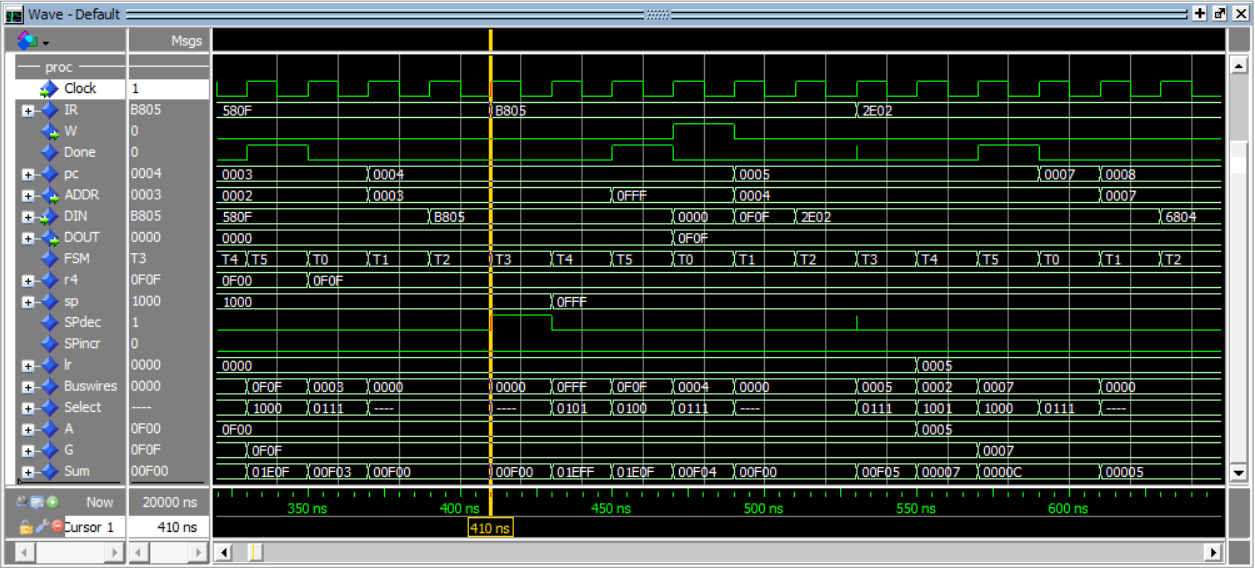
\includegraphics[width = .9\textwidth]{figures/push_bl.png}
    \end{center}
    \begin{center}
        \caption{Simulation results for code in Figure~\ref{fig:subr}. (Part $a$)}
        \label{fig:subr1}
    \end{center}
\end{figure}

\begin{center}
        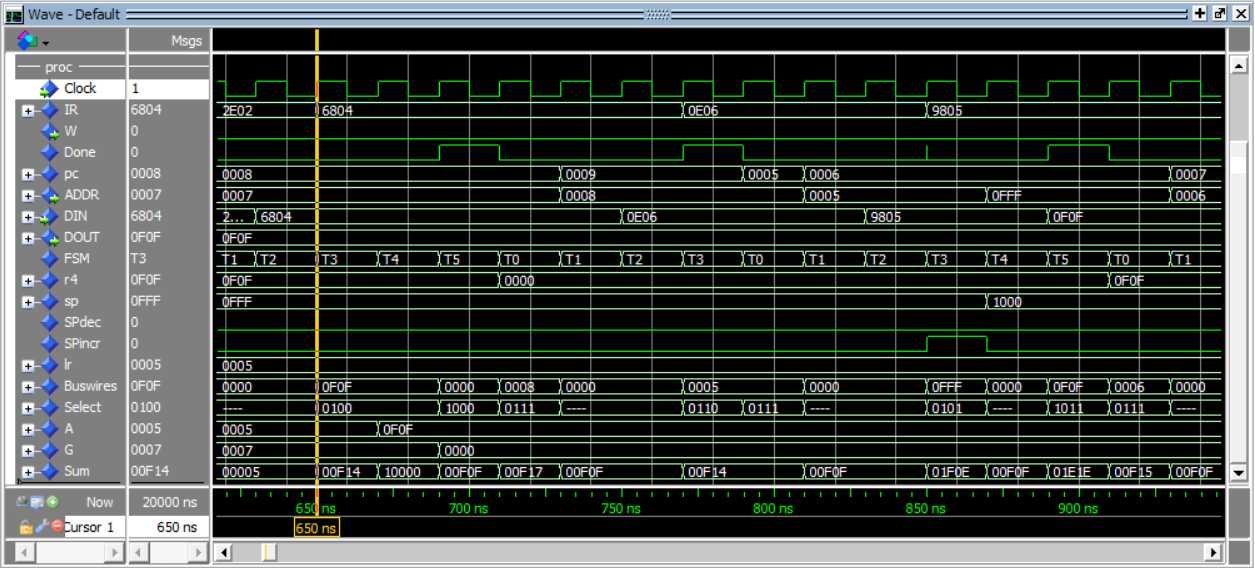
\includegraphics[width = .9\textwidth]{figures/bl_pop.png}
\end{center}

\begin{center}
Figure \ref{fig:subr1}: Simulation results for code in Figure~\ref{fig:subr}. (Part $b$)
\end{center}
\end{minipage}

~\\
~\\
An example of simulation results produced by executing the code in Figure~\ref{fig:subr} is
displayed in Figure~\ref{fig:subr1}. In part ($a$) of the figure 
the first two lines of code (three instructions) in the program have already been executed,
so that the stack pointer {\it sp} = 0x1000 and 
register $r4$ = 0x0F0F. At 410 {\it ns} in simulation time the processor loads the
instruction at address 3, which is \texttt{push~r4} (\texttt{0xb805}). 
As shown in the simulation results
the signal {\it sp\_decr} is asserted to decrement {\it sp} to \texttt{0xFFF}, and then
the contents of register $r4$ are written to the memory. At 530~ns in simulation time
the instruction \texttt{bl~SUBR} (\texttt{0x2E02}) is loaded into {\it IR}, from address 4. 
First, this instruction sets the link register {\it lr} to the value 5 (the subroutine return 
address), and then sets {\it pc} = 7, which is the address of \texttt{SUBR}. 

Figure~\ref{fig:subr1}$b$ continues the simulation results from Part ($a$). The first instruction 
of the \texttt{SUBR} subroutine, \texttt{sub~r4,r4} (\texttt{0x6804}), is loaded into 
{\it IR} at 650 {\it ns}. As shown in the simulation, this instruction results
in $r4$~=~0. Then, the subroutine
return instruction \texttt{mv~pc,lr} (\texttt{0x0E06}) is executed to return control to 
the address in {\it lr}, which is 5. The instruction at address 5 is \texttt{pop~r4}
(\texttt{0x9805}). It first reads from the memory at the address in 
{\it sp}, which is 0xFFF, and then asserts the {\it incr\_sp} signal, resulting in 
{\it sp} = 0x1000. Finally, the data read 
from the memory is used to restore the value $r4$ = 0x0F0F. 

\item Next, you should add the \texttt{cmp} instruction, which is similar to \texttt{sub}, as 
well as the shift and rotate instructions. Augment your ALU to include the barrel-shifter
capability illustrated in Figure~\ref{fig:barrel}. Simulation results for a
correctly-designed processor, executing code in Figure~\ref{fig:shift_code}, are displayed 
in Figure~\ref{fig:shift}.  In Part~($a$)
of the figure the first three instructions in the
code have already been executed, so that register $r0$~=~4 and $r4$~=~0x0F0F. 
At 350 {\it ns} in simulation time the processor fetches the instruction at address 3, which 
is \texttt{lsl~r4, \#1}. In time step $T_3$ of this instruction (which is indicated as
\texttt{011} in the waveform 
labeled {\it FSM}) register $r4$ is placed onto {\it Buswires} so that it can be copied into 
register $A$, in the ALU. Then, in time step $T_4$ the immediate data, which is 
in {\it IR} and specifies the shift amount, is placed onto {\it Buswires}. 
The {\it do\_shift} signal is asserted, so
that the ALU's {\it Sum} output is driven by the barrel shifter. It uses bits 3~-~0 from 
{\it Buswires} as the shift amount for the \texttt{lsl} instruction. The barrel shifter 
generates the result {\it Sum} = 0x1E1E, which is loaded into $r4$ at the end of
the instruction.

The next instruction executed in Figure~\ref{fig:shift}$a$ is \texttt{lsr~r4, \#1}. It
reverses the previous \texttt{lsl} operation, resulting in $r4$ = 0x0F0F. At 590 {\it ns}
in simulation time, the \texttt{lsl r4, r0} instruction is executed. Steps $T_0 -
T_3$ of this instruction appear in part ($a$) of 
Figure~\ref{fig:shift}, and the remaining time steps are
shown in Figure~\ref{fig:shift}$b$. Observe in time step $T_4$ that register $r0$ is
placed onto {\it Buswires}, because the shift amount (4) is contained in this register. 
This \texttt{lsl} instruction results in $r4$ = 0xF0F0. The final two instructions in the 
simulation are \texttt{asr r4, \#1}, which produces $r4$ = 0xF878, and \texttt{ror r4, r0},
which results in $r4$~=~0x8F87.


\lstset{language=ASM,numbers=none,escapechar=|}
\begin{figure}[H]
\begin{center}
\begin{minipage}[h]{9.5 cm}
\begin{lstlisting}[name=subr]
START:  mv    r0, #4
        mv    r4, =0x0F0F

        lsl   r4, #1        // lsl with Op2 = #D
        lsr   r4, #1        // lsr with Op2 = #D
        lsl   r4, r0        // lsl with Op2 = rY
        asr   r4, #1        // asr with Op2 = #D
        ror   r4, r0        // ror with Op2 = rY

END:    b     END
\end{lstlisting}
\end{minipage}
\caption{A program to test shift and rotate instructions.}
\label{fig:shift_code}
\end{center}
\end{figure}
\begin{minipage}[h]{15.5 cm}
\begin{figure}[H]
    \begin{center}
        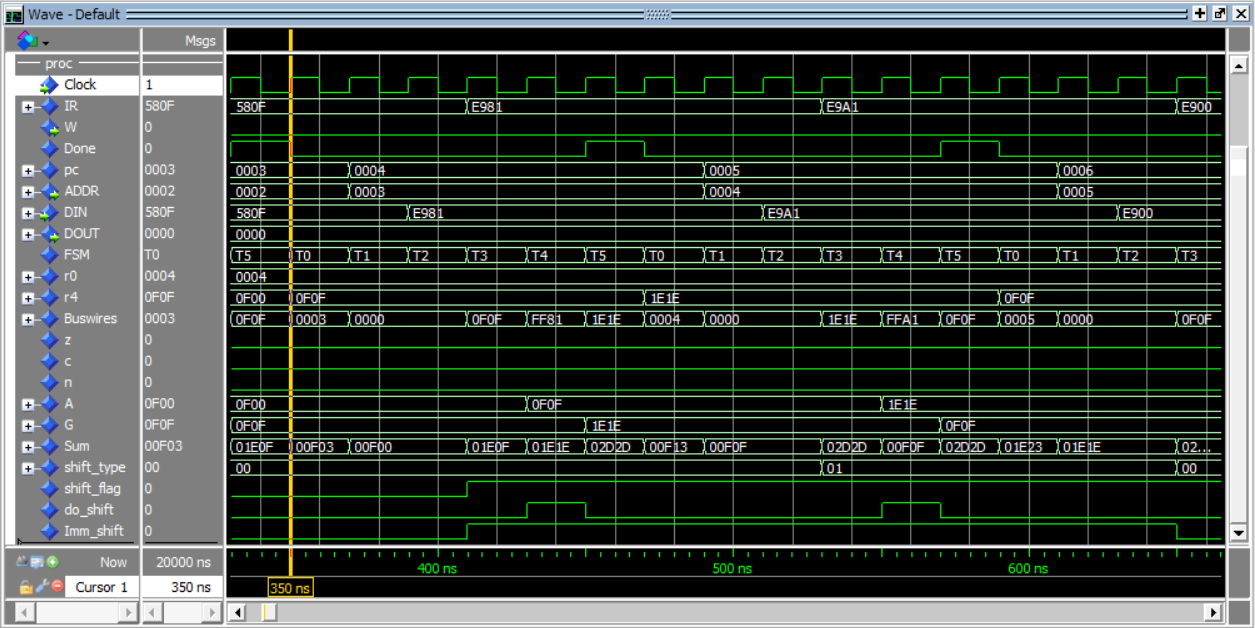
\includegraphics[width = .9\textwidth]{figures/shift_a.png}
    \end{center}
    \begin{center}
        \caption{Simulation results for code in Figure~\ref{fig:shift_code}. (Part $a$)}
        \label{fig:shift}
    \end{center}
\end{figure}

\begin{center}
        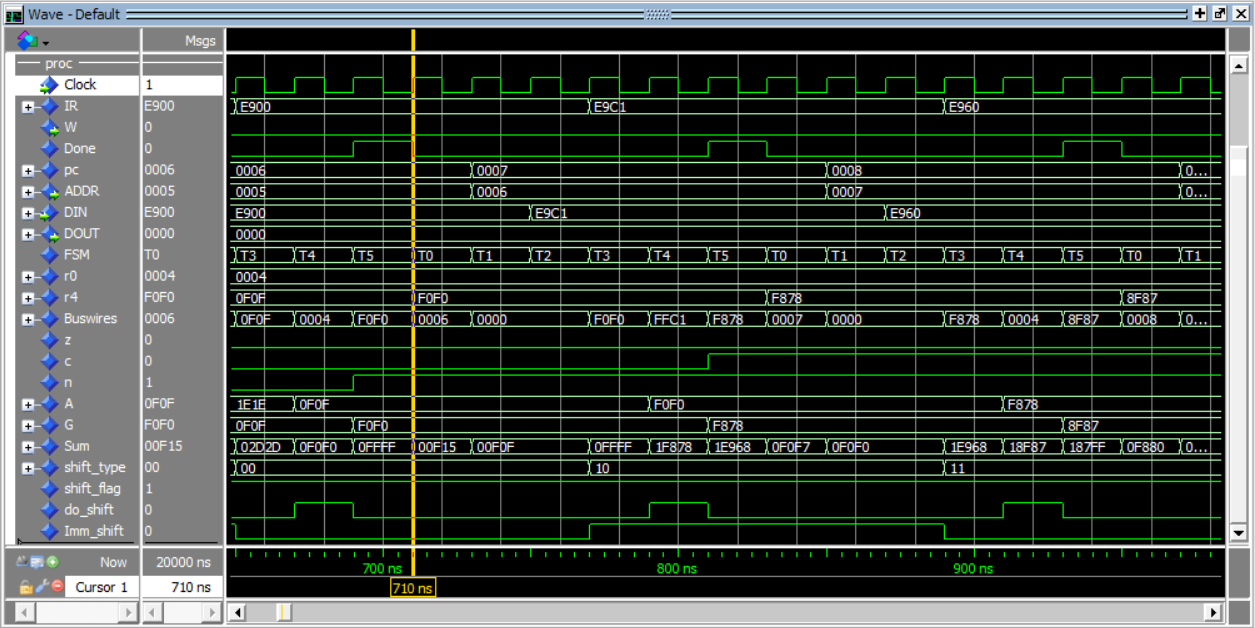
\includegraphics[width = .9\textwidth]{figures/shift_b.png}
\end{center}

\begin{center}
Figure \ref{fig:shift}: Simulation results for code in Figure~\ref{fig:shift_code}. (Part $b$)
\end{center}
\end{minipage}

~\\
\item An example of a subroutine, called \texttt{REG}, that you may find 
useful is given in Figure~\ref{fig:useful}. This subroutine is passed one parameter, 
in register $r0$. The purpose of the subroutine is to display the contents of this register, 
in hexadecimal, on \red{HEX3-0}. This code utilizes the \texttt{push}, 
\texttt{pop}, \texttt{cmp}, and \texttt{lsr} instructions, and also uses the {\it lr} to 
return from the subroutine.

A main program that calls the \texttt{REG} subroutine is provided in 
Figure~\ref{fig:shift_test}. This program tests the various shift and rotate operations,
as selected by the \texttt{SW} switches. The type of shift/rotate is chosen by setting the
switches \texttt{SW}$_{6-5}$ = 00 (\texttt{lsl}), 01 (\texttt{lsr}), 10 (\texttt{asr}),
or 11 (\texttt{ror}). The shift amount is chosen by setting \texttt{SW}$_{3-0}$. The
pattern shifted, $r0$ = 0xF0F0, is loaded at the start of the program. This pattern is
reloaded into $r0$ if a shift operation results in $r0$ = 0x0000 or $r0$ = 0xFFFF.

~\\
An assembly-language source-code file, called {\it shift\_test.s}, which includes the 
code in Figures~\ref{fig:useful} 
and~\ref{fig:shift_test} is provided as part of the design files for this exercise.
Assemble this code using {\it sbasm.py} and ensure that it works with your 
processor. As mentioned in Labs~9 and~10, you may want to make use of the DESim tool while
developing and debugging your processor. A video demonstration of the program in 
Figure~\ref{fig:shift_test} running on a correctly-working processor
using the {\it DESim} tool can be found at the URL:  

\noindent
\url{https://youtu.be/0k5GPGg_Vto}

\item Write some assembly-language code of your choosing that demonstrates the operations 
supported by your processor. You should make use of various I/O devices 
that are available to your processor, such as the \red{LEDR} lights, SW switches, 
and \red{HEX} displays.  In general, try to conceive of a program that does something
interesting and challenging. You should be able to demonstrate your code working properly
on a DE1-SoC, or similar board, but you may want to make use of {\it DESim} while
developing/debugging your code.

\lstset{language=ASM,numbers=none,escapechar=|}
\begin{figure}[H]
\begin{center}
\begin{minipage}[h]{12.5 cm}
\begin{lstlisting}[name=proc]
.define HEX_ADDRESS 0x2000

// subroutine that displays register r0 (in hex) on HEX3-0 
REG:   push  r1
       push  r2
       push  r3

       mv    r2, =HEX_ADDRESS  // point to HEX0

       mv    r3, #0            // used to shift digits
DIGIT: mv    r1, r0            // the register to be displayed
       lsr   r1, r3            // isolate digit
       and   r1, #0xF          // "    "  "  "
       add   r1, #SEG7         // point to the codes
       ld    r1, [r1]          // get the digit code
       st    r1, [r2]
       add   r2, #1            // point to next HEX display
       add   r3, #4            // for shifting to the next digit
       cmp   r3, #16           // done all digits?
       bne   DIGIT
       
       pop   r3
       pop   r2
       pop   r1
       mv    pc, lr

SEG7:  .word 0b00111111       // '0'
       .word 0b00000110       // '1'
       .word 0b01011011       // '2'
       .word 0b01001111       // '3'
       .word 0b01100110       // '4'
       .word 0b01101101       // '5'
       .word 0b01111101       // '6'
       .word 0b00000111       // '7'
       .word 0b01111111       // '8'
       .word 0b01100111       // '9'
       .word 0b01110111       // 'A' 1110111
       .word 0b01111100       // 'b' 1111100
       .word 0b00111001       // 'C' 0111001
       .word 0b01011110       // 'd' 1011110
       .word 0b01111001       // 'E' 1111001
       .word 0b01110001       // 'F' 1110001
\end{lstlisting}
\end{minipage}
\caption{A useful subroutine.}
\label{fig:useful}
\end{center}
\end{figure}

\lstset{language=ASM,numbers=none,escapechar=|}
\begin{figure}[H]
\begin{center}
\begin{minipage}[h]{13 cm}
\begin{lstlisting}[name=proc]
DEPTH 4096
.define LED_ADDRESS 0x1000
.define SW_ADDRESS  0x3000

START: mv   sp, =0x1000       // initialize sp

MAIN:  mv   r0, =0x9010
       bl   REG               // display r0 on HEX3-0
       bl   DELAY
LOOP:  mv   r1, =SW_ADDRESS
       ld   r1, [r1]
       mv   r2, =LED_ADDRESS
       st   r1, [r2]
       mv   r2, r1
       lsr  r2, #5            // get shift type (SW bits 6:5)

       cmp  r2, #0b00
       bne  LSR
       lsl  r0, r1
       b    CONT
LSR:   cmp  r2, #0b01
       bne  ASR
       lsr  r0, r1
       b    CONT
ASR:   cmp  r2, #0b10
       bne  ROR
       asr  r0, r1
       b    CONT
ROR:   ror  r0, r1

CONT:  bl   REG
       bl   DELAY

       cmp  r0, #0
       beq  MAIN
       cmp  r0, #-1
       beq  MAIN

END:   b    LOOP

// Causes a delay that works well when using DESim. For an actual 
// DE1-SoC board, use a longer delay!
DELAY: push r1
       mvt  r1, #0x04       // r2 <- 2^10 = 1024
WAIT:  sub  r1, #1
       bne  WAIT
       pop  r1
       mv   pc, lr
\end{lstlisting}
\end{minipage}
\caption{A program that test shift/rotate operations.}
\label{fig:shift_test}
\end{center}
\end{figure}

\end{enumerate}
\end{document}
